\documentclass[tikz,border=5pt]{standalone}

\usepackage{tikz}

\begin{document}

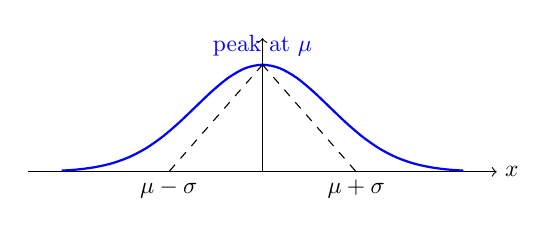
\begin{tikzpicture}[scale=0.85, transform shape]
  \draw[->] (-3.5,0) -- (3.5,0) node[right]{$x$};
  \draw[->] (0,0) -- (0,2.0);

  \draw[domain=-3:3, smooth, thick, blue]
    plot (\x, {1.6*exp(-\x*\x/2)});

  \draw[dashed] (0,1.6) -- (-1.4,0) node[below]{$\mu - \sigma$};
  \draw[dashed] (0,1.6) -- ( 1.4,0) node[below]{$\mu + \sigma$};

  \node[blue, above] at (0,1.6) {peak at $\mu$};
\end{tikzpicture}

\end{document}
